\section{Introduction}
\label{ch:intro}

After so many years and so many games, online games are still so popular that the end is nowhere in sight.
Millions buy not just the latest software and games but also the environment, such as PCs and consoles just to play their favorite games at their best.
For them, the most terrifying thing is when they encounter cheaters in the game.
Of course it is bad if you lose in the game or cannot complete the mission, but the game itself can be destroyed if there are a lot of hackers and cheaters.
This work shows how game developers can prevent cheaters from appearing in the game and thereby save their product.

Filtering out the cheaters is not new. 
There is a lot of work, research which processes this problem and try to show how the developers can defend against it.
% PROBLEM
The exact definition of our problem is that the gaming industry can not keep up with modern cheaters, and cheat developers, therefore there are several ways to cheat in recently popular games, no matter how strong the applied anti-cheat method is. 
In our paper, we will go through the best current methods available for game developers and using that information we will try to provide a new solution for filtering out the cheating users.
We also show what the biggest drawbacks of the aforementioned researches are, why our solution is able to fill these holes and at the same time we prove why our innovation can do more than the others.

Our solution uses AI technologies such as Convolutional Neural Networks, Cross-validation, Deep Neural Networks, Explainable AI, K-Nearest Neighbour.
With our innovation we are making profiles and generate scores for the user actions, with the mentioned AI technologies, and filtering out the potentially engaged users in cheating activity. 
We also try to cover as many online game type as possible with our system. We are trying to provide a detector app that knows after a very short time if there is a cheater in the game.

With this research we are hoping to help the game developers to develop safer games and to provide more stable games for those, who are love games, who are like to play online games.
We presented this work to show that cheaters are still a problem to the gaming community, and to show that there are ways to prevent their negative impact on the gaming industry.
We are hoping that with this work, we can help to reduce the cheating users in game, and also we hope that more and more new game developers and their new games will appear, because they can develop fast and effective cheat detection to their system, which saves their product from the cheaters.

\begin{figure}[h]
\centering
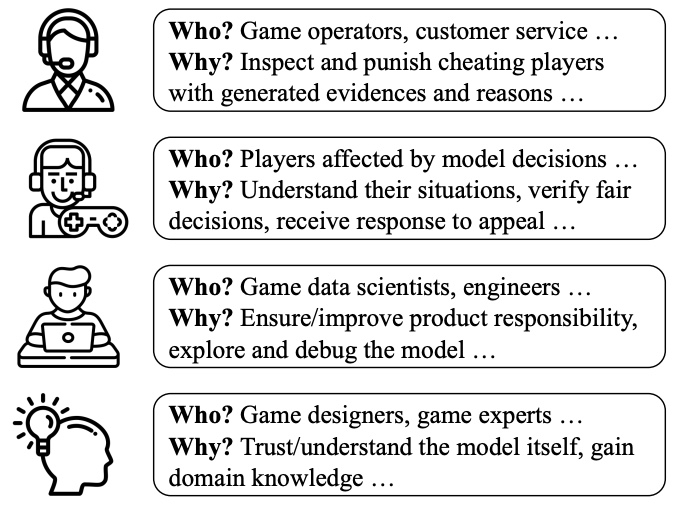
\includegraphics[width=0.4\linewidth]{contents/images/purpose.jpeg}
\captionsetup{width=0.4\textwidth}
\caption{\label{fig:purpose}Diagram showing the different purposes of explainable game cheating detection sought by different audiences.}
\end{figure}

The structure of the paper is as follows: \Cref{ch:lit_rev} contains the most important papers of the topic with a short review about their work and their relevance to our research.
% \Cref{ch:background} provides further information on the topic.
\Cref{ch:methodology} provides our method for cheat detection and a few examples why it works and why it is better than the current methods.
In \Cref{ch:discussion} we discuss our findings and talk about the results of our research.
\Cref{ch:conclusion} concludes the results of our research.
\Cref{ch:future} depicts possible further future work on this topic and on our system.